\documentclass[12pt,english]{article}
\usepackage[a4paper,bindingoffset=0.2in,%
            left=1in,right=1in,top=1in,bottom=1in,%
            footskip=.25in]{geometry}
\usepackage{graphicx}
\usepackage{listings}
\usepackage{float}
\usepackage{hyperref}

% \graphicspath{{./res/}}
\begin{document}

\begin{center}
\textbf{{\large Proiect Baze de Date}}

{\footnotesize{Pangratie Andrei}}
\end{center}

\paragraph{ Proiectarea bazei de date }

\begin{flushleft}
Mai jos este schema bazei de date. Sunt doua parti ale bazei de date. Partea in care sunt retinuti angajatii si utilizatorii site-ului si partea in care sunt retinute comenzile.
Angajatii sunt impartiti in doua categori: ospatari si manageri. Managerii au dreptul de a adauga alti ospatari sau manageri. Atat ospatarii cat si managerii sunt utilizatori, diferenta intre ei este facuta de drepturile de pe site. Exista utilizatori care nu sunt nici manageri, nici ospatari, acestia au doar dreptul de a face comenzi acasa si de a naviga partile publice ale site-ului. 
\end{flushleft}

\begin{figure}[H]
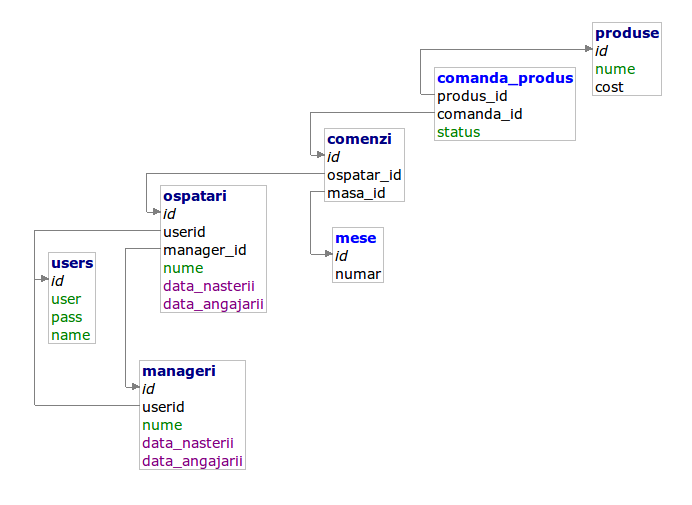
\includegraphics[width=1\textwidth]{schema.png}
\caption{Schema bazei de date}
\end{figure}

\paragraph{ Interfata site-ului }

\begin{flushleft}
Pagina de login si cea de sign up este deschisa persoanelor in general si este folosita si de angajatii restaurantului. Angajatii restaurantului au dupa caz drepturi in plus (ospatarii controleaza comenzile, managerii controleaza atat comenzile cat si rolul utilizatorilor). Angajatilor le este luata pagina de livrari.
\end{flushleft}

\begin{figure}[H]
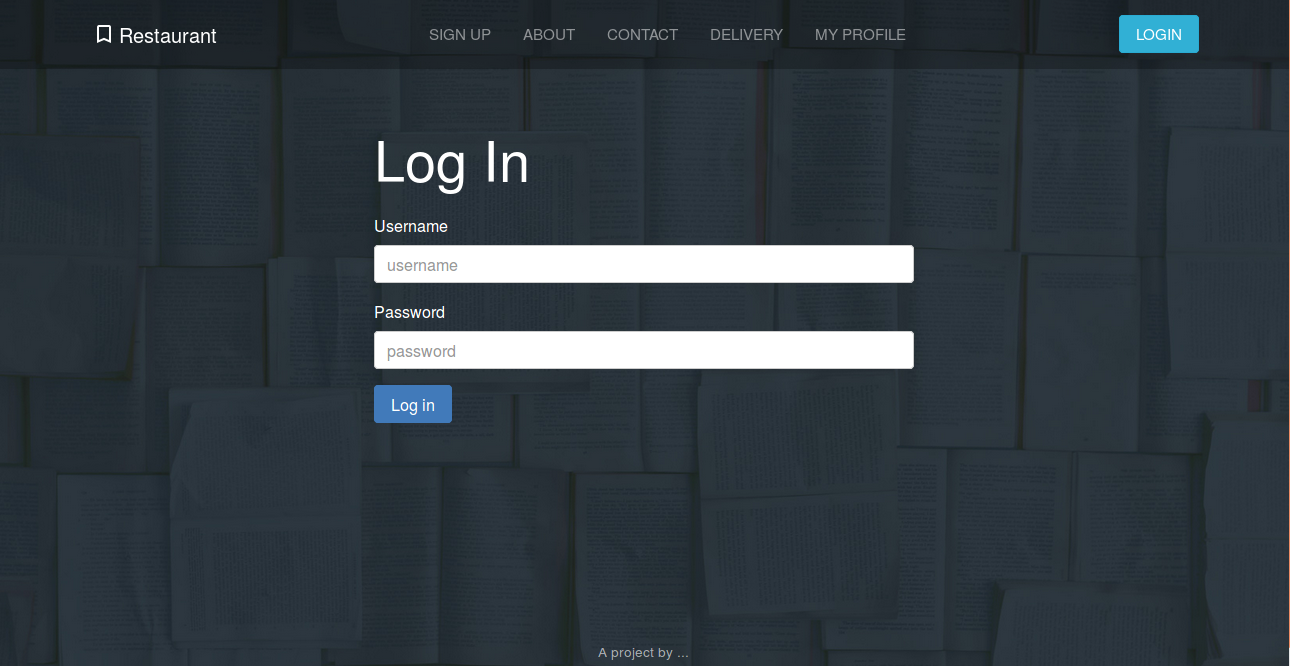
\includegraphics[width=1\textwidth]{login.png}
\caption{Pagina Login}
\end{figure}

\begin{figure}[H]
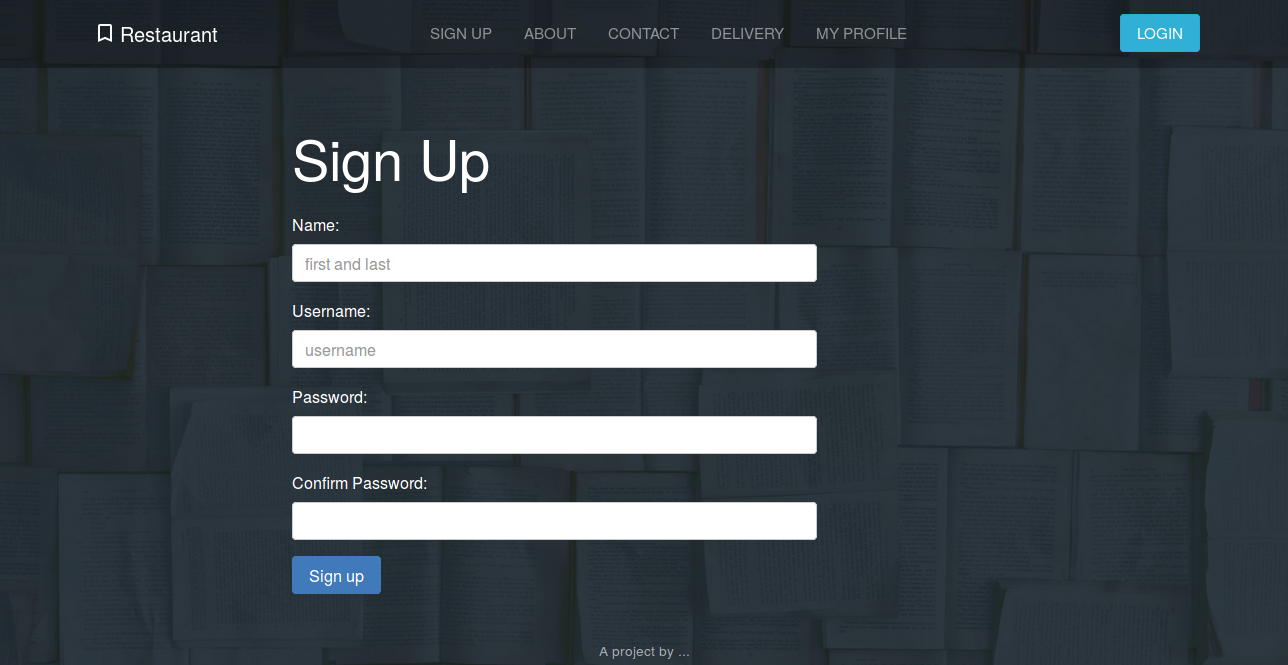
\includegraphics[width=1\textwidth]{sign_up.png}
\caption{Pagina Sign Up}
\end{figure}

\begin{flushleft}
Adminul are 6 controale asupra angajatiilor: el poate lista managerii si ospatarii,
poate sa faca un utiliator sa fie manager sau ospatar sau poate sa ia dreptul unui utilizator de a fi manager sau ospatar. 
\end{flushleft}

\begin{figure}[H]
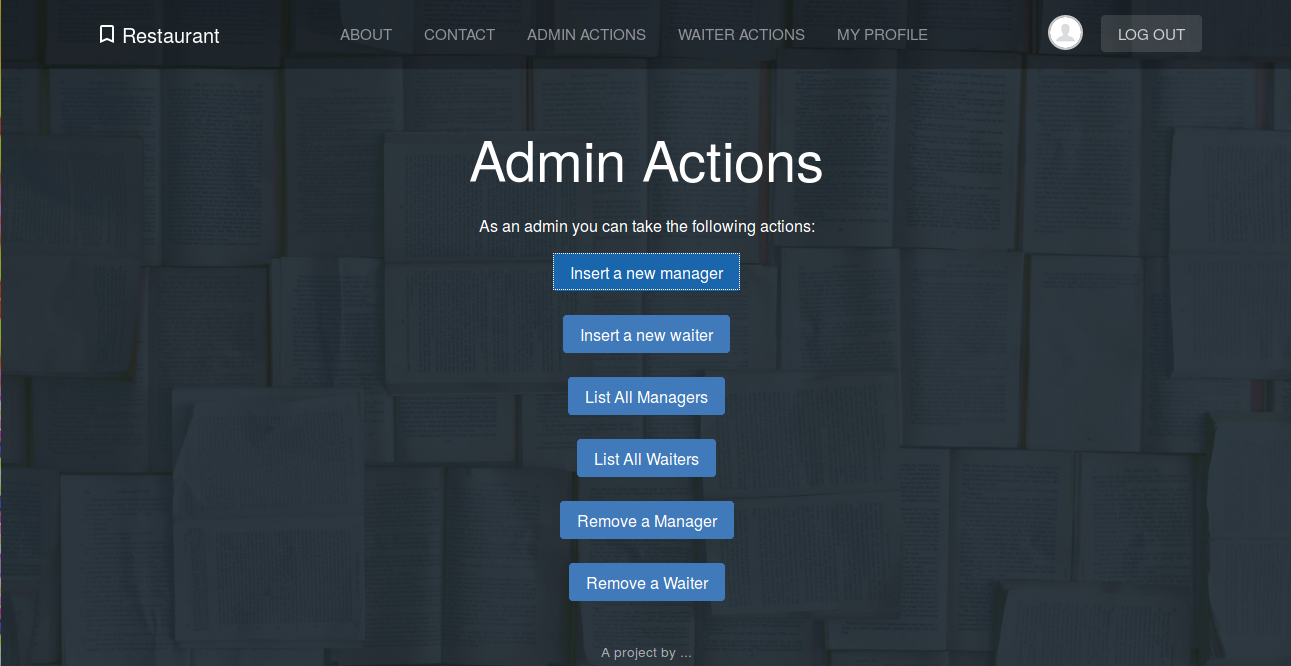
\includegraphics[width=1\textwidth]{admin_1.png}
\end{figure}

\begin{figure}[H]
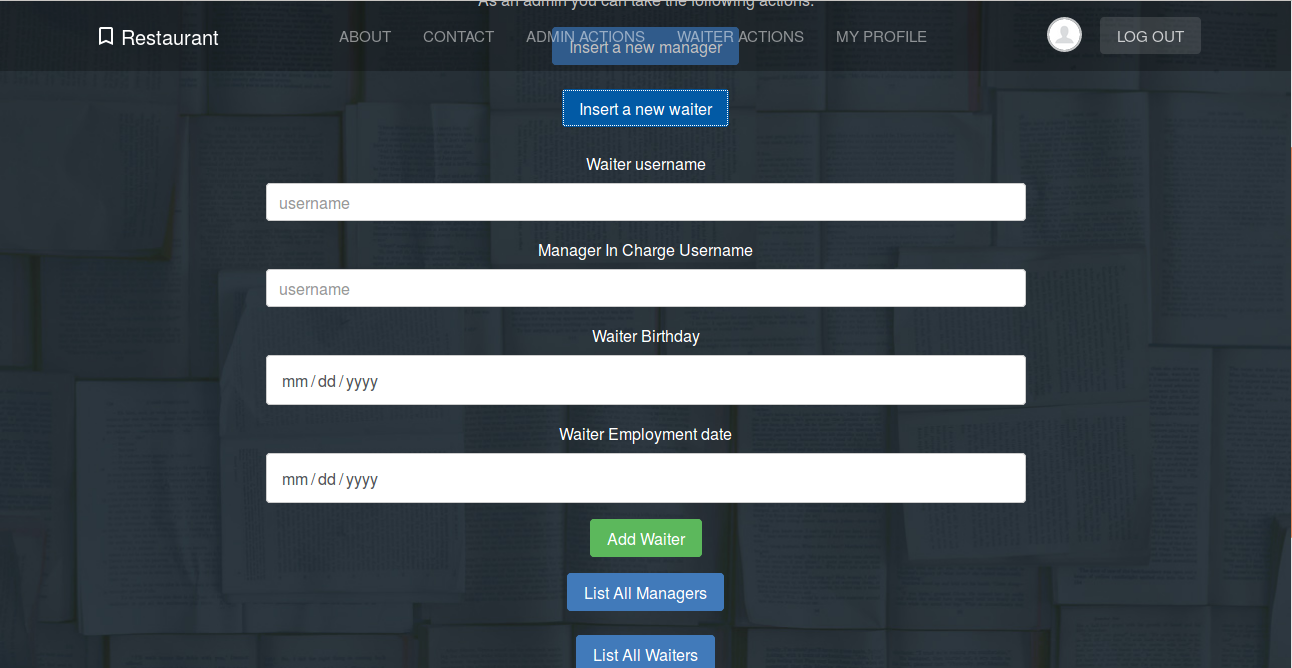
\includegraphics[width=1\textwidth]{admin_2.png}
\end{figure}

\begin{figure}[H]
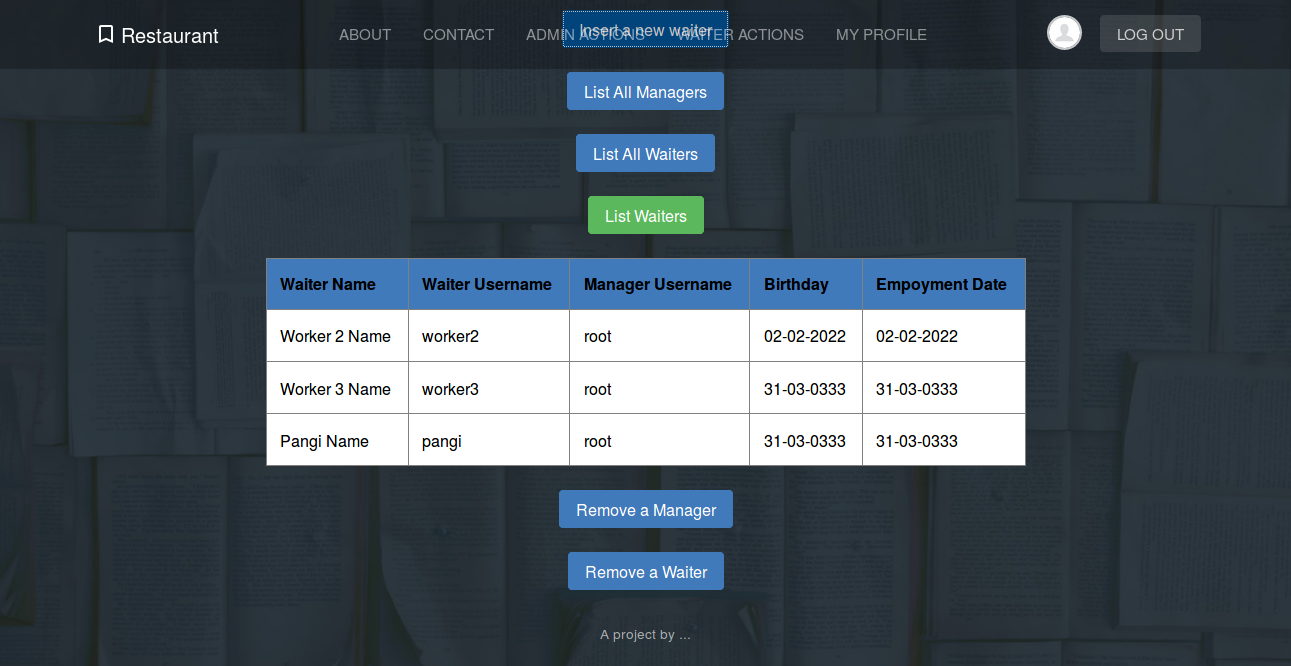
\includegraphics[width=1\textwidth]{admin_3.png}
\end{figure}

\begin{figure}[H]
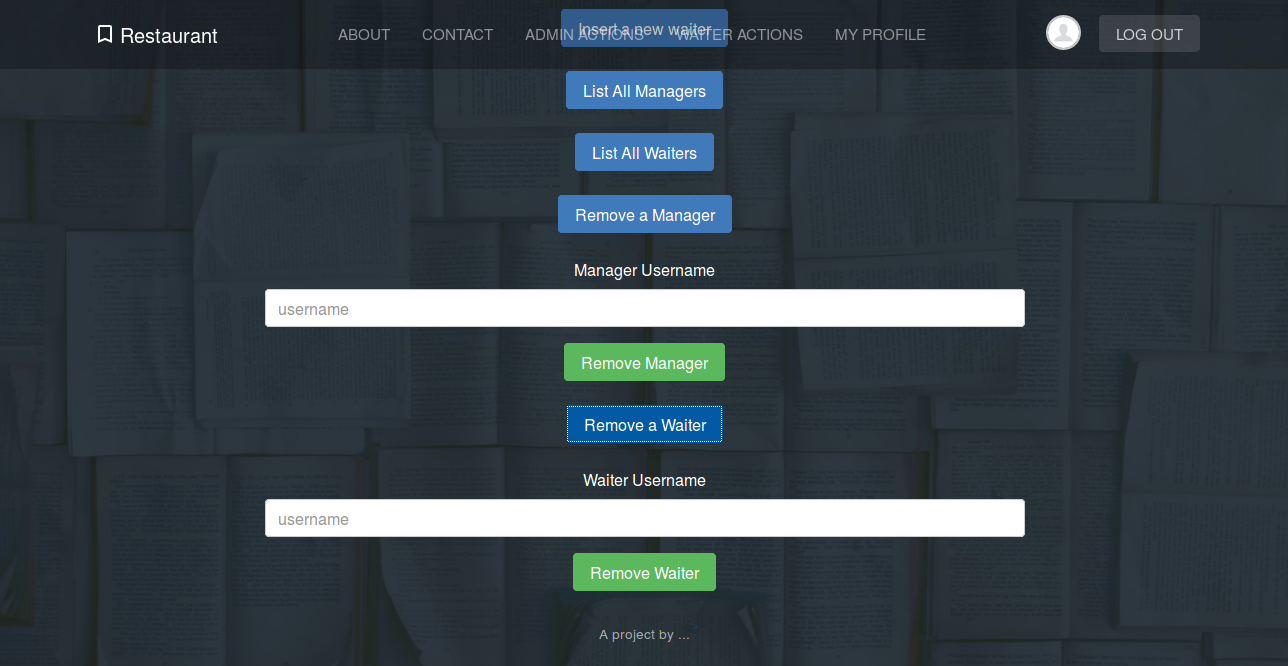
\includegraphics[width=1\textwidth]{admin_4.png}
\end{figure}

\begin{flushleft}
[neterminat] Ospatarii pot sa introduca comenzi, astfel ei pot sa introduca mai multe produse si numarul unei mese si vor forma o comanda. Comanda va fi listata impreuna cu un numar unic printre comenzile actuale pe pagina. Ospatarul va putea lua o comanda dupa ce este terminata si va putea sa o duca la masa respectiva, stergand-o din lista de comenzi. Ospatarul va putea introduce produse noi si va putea scoate produsele vechi din lista de comenzi.
\end{flushleft}

\begin{figure}[H]
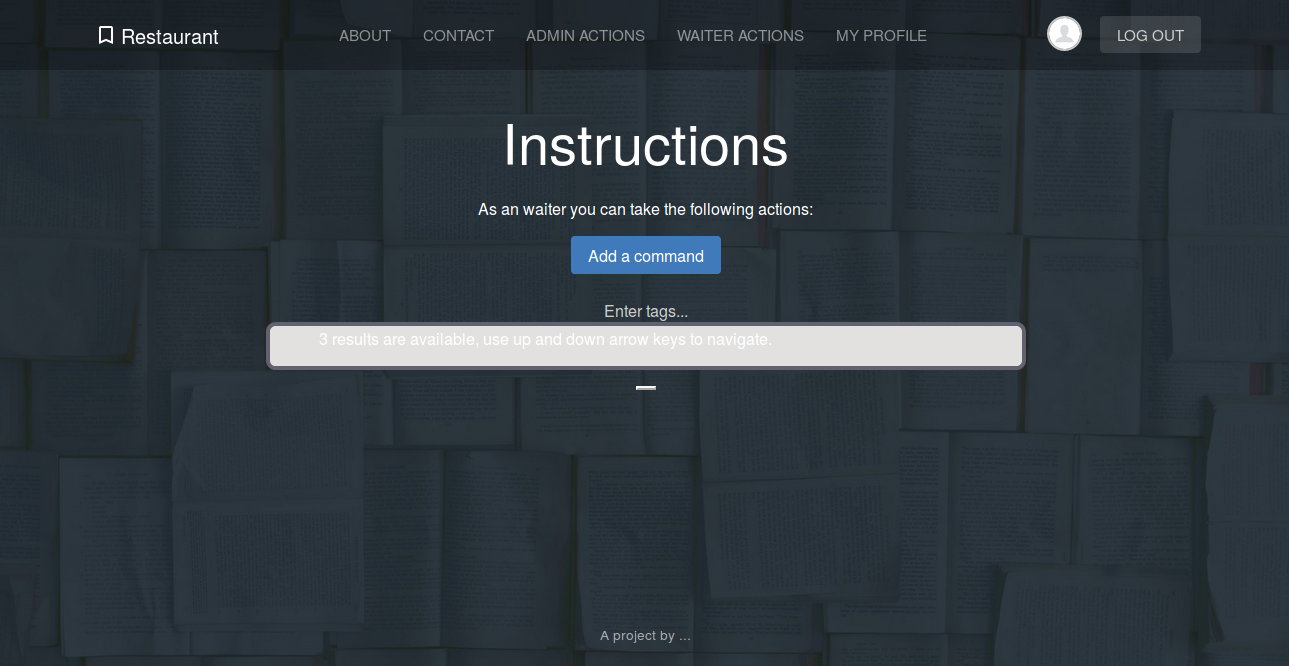
\includegraphics[width=1\textwidth]{waiter_1.png}
\end{figure}

\paragraph{ Logica interna a bazei de date }

\begin{flushleft}
Pentru a decide nivelul de privilegiu al userului curent (manager/admin, ospatar/muncitor, oaspete) se folosesc urmatoarele interogari in baza de date:

\end{flushleft}
\begin{lstlisting}
select * 
    from users user, manageri manager
        where user.id = manager.userid
                and user.user = \"${username}\"
\end{lstlisting}

\begin{flushleft}
Pentru a vedea daca userul curent este un manager.
\end{flushleft}

\begin{lstlisting}
select * 
    from users user, ospatari ospatar
        where user.id = ospatar.userid
                and user.user = \"${username}\"
\end{lstlisting}

\begin{flushleft}
Pentru a vedea daca userul curent este un ospatar.
\end{flushleft}

\begin{flushleft}
Pentru a afla daca exista un manager care sa aiba numele de utilizator introdus la adaugarea unui ospatar se foloseste urmatoarea interogare:
\end{flushleft}

\begin{lstlisting}
select manager.id
    from manageri manager, users user
        where user.user = \"${manager_username}\"
            and manager.userid = user.id limit 1`
\end{lstlisting}

\begin{flushleft}
Pentru a obtine tabela cu ospatarii se foloseste:
\end{flushleft}

\begin{lstlisting}
select
    waiter.nume as name,
    waiter.data_nasterii as birthday,
    waiter.data_angajarii as employment_date,
    waiter_user.user as waiter_username,
    manager_user.user as manager_username
from ospatari waiter
    join manageri manager on manager.id = waiter.manager_id
    join users waiter_user on waiter_user.id = waiter.userid
    join users manager_user on manager_user.id = manager.userid
\end{lstlisting}

\begin{flushleft}
Pentru tabela cu managerii se utilizeaza:
\end{flushleft}

\begin{lstlisting}
select
    manager.nume as name,
    manager.data_nasterii as birthday,
    manager.data_angajarii as employment_date,
    manager_user.user as manager_username
from manageri manager
    join users manager_user on manager_user.id = manager.userid
\end{lstlisting}

\begin{flushleft}
Pentru a sterge un manager cu un anumit nume de utilizator s-a folosit:
\end{flushleft}

\begin{lstlisting}
delete manager from manageri manager
    where manager.userid = 
        (select manager_user.id from users manager_user
            where manager_user.user = \"${manager_username}\")
\end{lstlisting}

\begin{flushleft}
Asemanator pentru a sterge un anumit ospatar:
\end{flushleft}

\begin{lstlisting}
delete waiter from ospatari waiter
where waiter.userid = 
    (select waiter_user.id from users waiter_user
        where waiter_user.user = \"${waiter_username}\")
\end{lstlisting}

\paragraph{ Fisierul README: }

\begin{center}
\lstinputlisting{../README.md}
\end{center}

\begin{flushleft}
Link direct catre site:
\end{flushleft}

\begin{center}
\href{http://ec2-35-180-32-243.eu-west-3.compute.amazonaws.com:7555}{Link site}
\end{center}

\end{document}
